%=== CHAPTER ONE (1) ===
%=== INTRODUCTION ===

\chapter{Introduction}
\begin{spacing}{1.5}
\setlength{\parskip}{0.3in}

This chapter describes the background of the problem that will be focused on. \autoref{sec:IN_background} will describe the scene where intelligent car driving and ADAS system are applied and state the importance of lane and road marking detection in the ADAS system. \autoref{sec:IN_motivation} will explain why such problems should be solved and on which specific issues this dissertation will be focusing. \autoref{sec:IN_objectives} will give the objectives and the scope of this dissertation. \autoref{sec:IN_contribution} will briefly introduce my contributions in this work. \autoref{sec:IN_organisation} will give the outline of the following chapters.

\section{Background}
\label{sec:IN_background}

This section will explain the background of the intended problems. It will describe how smart cars assist human drivers by using the Advanced-driver-assistance system (ADAS) system and how object-detection methods help the ADAS system perform better.

The era of intelligent cars is coming, and the Advanced-driver-assistance system plays an essential role in it. Object detection technologies are used to improve the performance of Advanced-driver-assistance systems.

Smart cars equipped with an Advanced-driver-assistance system are popular now. With smart driving and Eco-energy technology development, more and more companies began producing and selling the newly designed, electric-driven, smart-driving assistant cars. Leading companies like TESLA, NIO, and QuantumScape made hundreds of thousands of cars every year (till 2020)~\cite{petranek2015we}. With these cars bought by more and more families, smart cars are no longer a concept for ordinary people. However, they become daily necessities for everyone, as an alternative to a traditional car. Compared with traditional mechanical fuel vehicles, new intelligent vehicles have many advantages. They are 'new' not only because they are driven by electric energy but also because they are equipped with intelligent driving assistance systems, usually called the Advanced-driver-assistance system (ADAS).


\begin{figure}[ht]
\centering
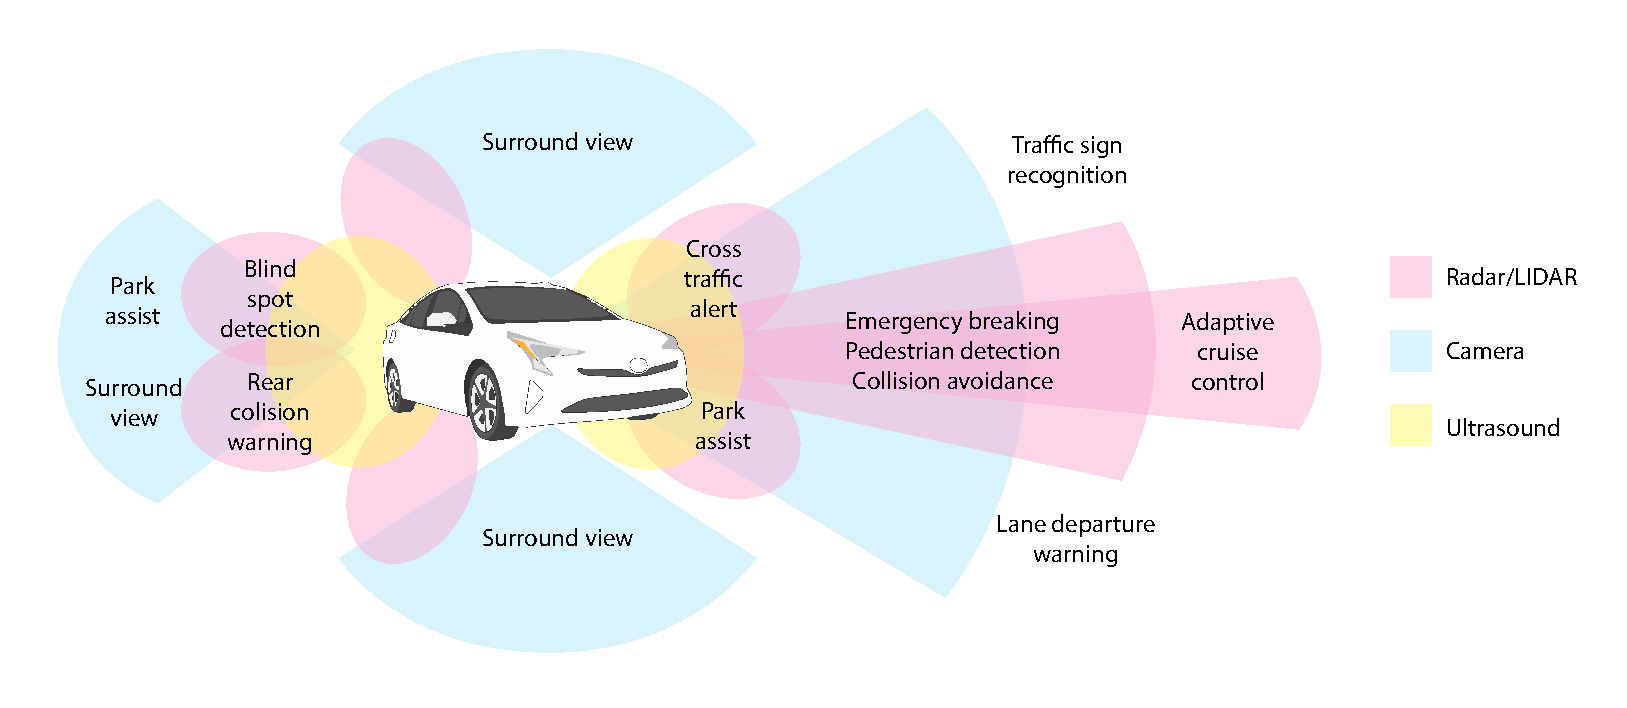
\includegraphics[width=0.99\textwidth, fbox]{Chapter1/adas.pdf}
\caption{Advanced Driver Assistance System (ADAS)~\cite{adas}}
\label{fig:adas} 
\end{figure}

ADAS system can reduce road fatalities by minimizing human error. The basic architecture of the ADAS system can be shown in \autoref{fig:adas}. Firstly, it utilizes the sensors (LIDAR, in-vehicle camera, GPS) to collect the surrounding obstacle or global position information. Secondly, by combining the information grabbed from all the sensors, the ADAS system can get valuable information for driving, such as driver's state, current geographical position of cars, road congestion, potential obstacles on the road, and trending road~\cite{morignot2014arbitration}. The driver or the analysis system can further utilize such information to avoid potentially dangerous. Because the safety problem is one of the most severe unsolved problems of the traditional human-controlled vehicles, ADAS can significantly reduce the death rate related to fatal driving~\cite{brookhuis2001behavioural}.

To improve the performance of the ADAS system is an object detection task. ADAS systems use in-vehicle cameras to capture the real-time images of roads~\cite{ziebinski2016survey}. Captured images will be handled by a detection module that recognizes lane outlines and road markings and then responds to drivers accordingly. This recognizing algorithm is an object detection problem in the computer vision area. 

This dissertation work wants to solve the problems raised in the aforementioned background. The lane-detection method described in this report can be used to improve the ADAS system's performance. 

\section{Motivation}
\label{sec:IN_motivation}

This section will explain why such research is essential. It describes the specific problems that will be solved. Example images in this section are selected from VPG data set~\cite{lee2017vpgnet}.

There are several common lane detection issues in the aforementioned detection process. Two important ones are bad surrounding conditions and the curved road.

First is rainy and lousy illumination conditions. On rainy days, images captured by ADAS’s camera may be blurry or be stained by raindrops as in \autoref{fig:blurry}, and the water on the road may lead to reflection of lights, as shown in \autoref{fig:reflection}. At dusk, the sun is dim, and the scene is dark-some. The road markings and lane outlines cannot be distinguished from the background easily, as shown in~\autoref{fig:dusk} (in the dusk) and \autoref{fig:night} (in the night). With such distortions, the detection algorithm cannot see roads accurately. There are two approaches to address bad weather problem: 1) denoise the raindrops first in pre-processing and do detection later; 2) use domain-critical information to better guide the detector to see features native to this extreme weather case. In this dissertation, the second approach is applied.


\begin{figure}[th]
    \centering
    % \begin{adjustbox}{minipage=0.98\linewidth,fbox}
    \begin{subfigure}[b]{0.49\textwidth}
        \centering
        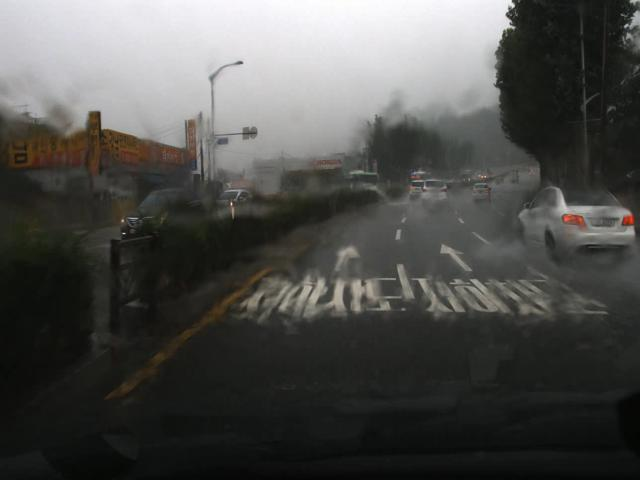
\includegraphics[width=2.7in, fbox]{Chapter1/blurry.png}
        \caption{Blurry Sample}
        \label{fig:blurry} 
    \end{subfigure}%
    ~
    \begin{subfigure}[b]{0.49\textwidth}
        \centering
        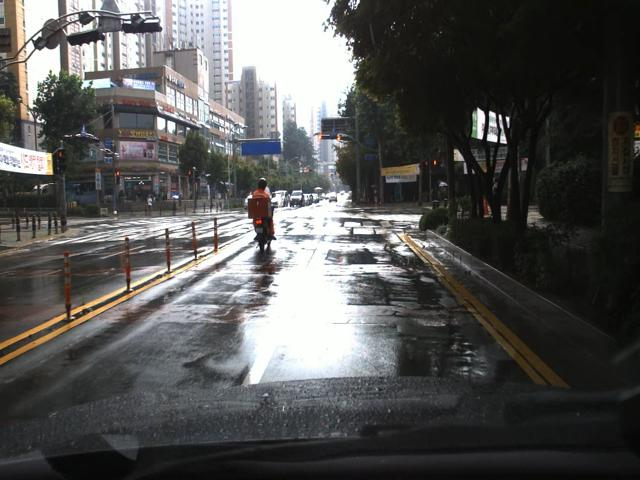
\includegraphics[width=2.7in, fbox]{Chapter1/reflection.png}
        \caption{Reflection Sample}
        \label{fig:reflection} 
    \end{subfigure}
    \\
    \begin{subfigure}[b]{0.49\textwidth}
        \centering
        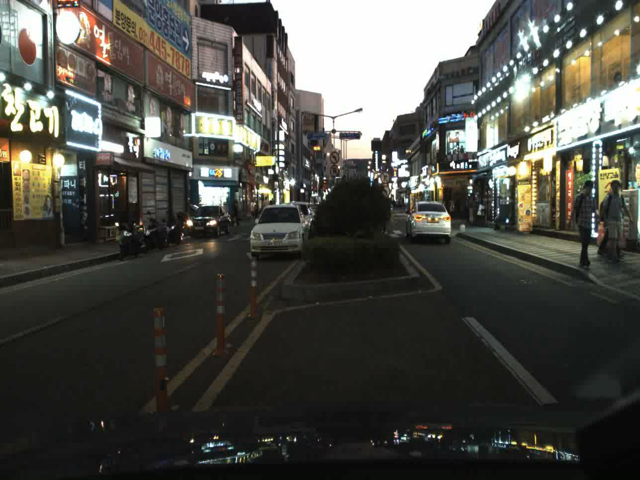
\includegraphics[width=2.7in, fbox]{Chapter1/dusk.png}
        \caption{In the Dusk}
        \label{fig:dusk} 
    \end{subfigure}%
    ~
    \begin{subfigure}[b]{0.49\textwidth}
        \centering
        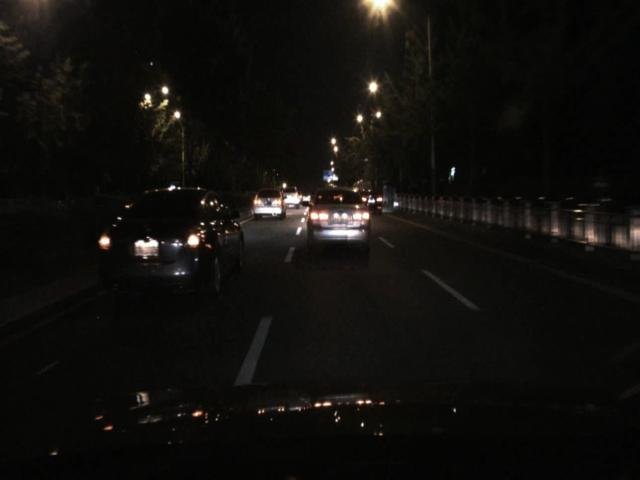
\includegraphics[width=2.7in, fbox]{Chapter1/night.png}
        \caption{In the Night}
        \label{fig:night} 
    \end{subfigure}
    % \end{adjustbox}
    \caption{Rainy and Bad Illumination Condition}
\end{figure}

The second is the curved road. Traditional lane detection algorithms usually work well on the straight lane but will meet performance drop once the road turns quickly. The comparison of straight road and curved road can be seen in \autoref{fig:straight} and \autoref{fig:curved}.

\begin{figure}[th]
    \centering
    \begin{subfigure}[b]{0.49\textwidth}
        \centering
        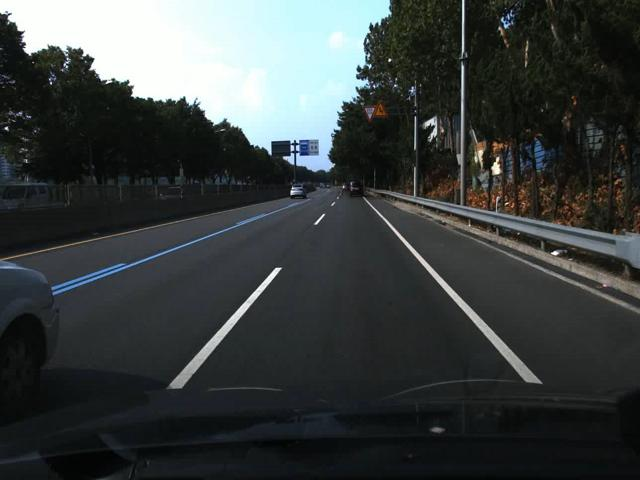
\includegraphics[width=2.7in, fbox]{Chapter1/straight.png}
        \caption{Straight Lane}
        \label{fig:straight} 
    \end{subfigure}%
    ~
    \begin{subfigure}[b]{0.49\textwidth}
        \centering
        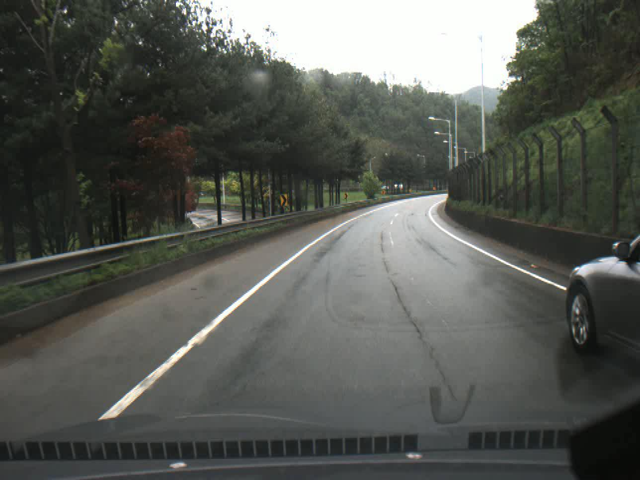
\includegraphics[width=2.7in, fbox]{Chapter1/curved.png}
        \caption{Curved Lane}
        \label{fig:curved} 
    \end{subfigure}
    \caption{Straight and Curved Lane}
\end{figure}

VPGNet~\cite{lee2017vpgnet} used vanishing point information to solve this problem. The vanishing point is the visual intersection of two parallel lines~\cite{barnard1983interpreting}, here it is treated as the unseen end of the road.  Inspired by the intuition that human eyes utilize the vanishing point to predict the road trending, VPGNet tried to feed this information into the neural network by the multi-task method. They use multi-task because features employed by VP task, like road curving angle and trending, may also be helpful in the detection of lanes and road markings. Based on this, we can expect that with VP information given, the Neural Network can converge better on the other two tasks (lane detection, road marking detection). However, VPGNet’s VP feeding scheme is simple, not as efficient as expected. In this dissertation, a new scheme to train with VP information was proposed.

The motivation of this research work is to solve the above-mentioned problems. The ADAS system can perform better in lane detection and road marking recognition by solving those problems, making auto-driving safer.

\section{Objectives and Specifications}
\label{sec:IN_objectives}

This project aims at developing a Neural Network architecture that can detect the lanes and the road markings from the images. The images are captured by in-vehicle cameras. The input is 3-channel RGB image, and the output is a pixel-level classification of the objects in the target image. There are 17 classes of objects, as being listed in \autoref{tab:classes}. Besides, it will predict the vanishing point, which will also guide the curving lane's prediction. The architecture was implemented both in Caffe and PyTorch.

The training data mainly comes from two sources. The first is the VPG data set~\cite{lee2017vpgnet}, and the second is the Caltech data set~\cite{aly2008real}.

\section{Major contributions of the Dissertation}
\label{sec:IN_contribution}

This dissertation researched a pixel-level lane detection and road marking classification Neural Network architecture based on the Fully Convolution Network and multi-task training method. It employs the vanishing points to improve the performance of the lane detection and road marking classification accuracy. The network is implemented in both Caffe~\cite{jia2014Caffe} framework in C++ and PyTorch~\cite{NEURIPS2019_9015} framework in Python3~\cite{python3}.

In the data pre-processing, a data format transition algorithm between the two lane data sets (VPG data set \cite{lee2017vpgnet} and Caltech data set \cite{aly2008real}) was implemented. Thus the two data set can be translated into the same data format, by which format can be fed into either the Caffe or the PyTorch framework. A multi-class visualization algorithm is proposed in the data post-processing, which gives each class distinguishable colour and annotates each pixel with its corresponding colour.

In the network architecture part, two brand new combination layers are described. One is the tilling layer which works as an alternative to the traditional concatenate layer with more efficiency. Another one is the N-map combination layer which feeds the Vanishing Points to the model. The network is implemented in both Caffe and PyTorch. $2-D$ Gaussian functions are also used to enhance the prediction of the vanishing points.

After the training process, the confidentiality threshold is discussed, which will affect the model's efficiency when applied in practice.

\section{Organisation of the Dissertation}
\label{sec:IN_organisation}

The following chapters will be organized into six chapters: Literature Review, Vanishing Point Directed Lane Detection, Improvements, Experimental Results and Discussion, Conclusion and Recommendations.

{\large\textbf{Chapter 2: Literature Review}}

\autoref{cha:literature} will review some of the background theories and algorithms related to object detection in lane and road marking recognition. \autoref{sec:LR_overview} will give an overview of the history of deep learning networks used in object detection. \autoref{sec:LR_FCN} will describe the basic theory of Fully Convolution Network and its working mechanism. 
% In \autoref{sec:LR_objectdetection} I discussed the history of object detection algorithms and introduced some famous ones. 
% In \autoref{sec:LR_vpinNN} I introduced Vanishing Point's concept and its usage in other lane detection tasks.

{\large\textbf{Chapter 3: Refined VP Guided Lane Detection Network: RVPGNet}}

\autoref{cha:model} will introduce the network architecture of my proposed Neural Network and the detailed specifications in training. \autoref{sec:MD_model} will introduce the main network structure and its multi-task configuration. \autoref{sec:MD_Caffe} will introduce the Caffe implementation's training process, its environment configuration, and some user-defined layers used. \autoref{sec:MD_PyTorch} will introduce the PyTorch implementation of this network and the data transition procedure. \autoref{sec:MD_2D} will introduce a new improvement to feed the training data: the $2-D$ Gaussian feeding. It will introduce the mathematical theory of $1-D$ and $2-D$ Gaussian functions and explain why the training should be more efficient in this way.

{\large\textbf{Chapter 4: Experimental Results and Discussion}}

 \autoref{cha:experiments} will discuss the model's experiment results. It gives the mathematical equations of the test metrics. After that, it will introduce a visualization tool that can be used to annotate the pixel-level classification images. Then, the experimental outputs in a normal situation and rainy situation are analyzed. Finally, it will discuss the confidential threshold selection of the prediction result.

{\large\textbf{Chapter 5: Conclusion and Recommendations for Future Work}}

\autoref{cha:conclusion} will summarize the entire work. It will give the conclusion of experimental results and also the conclusion of work that has been done. It also gives some future work recommendations in the last section.

\end{spacing}
%=== END OF CHAPTER ONE ===
\newpage


